% Definition der Klasse des Dokumentes
\documentclass[11pt, a4paper]{article}

\usepackage[T1]{fontenc}        % Sorgt u.a. dafür, dass Texte vernünftig markierbar werden auch bei Sonderzeichen
\usepackage{ae,aecompl} %bessere Schrift
\usepackage{gensymb}
\usepackage[ngerman]{babel}     % Deutsches Wörterbuch usw.
\usepackage{epstopdf}   % Wandelt .eps Dateien automatisch um
\usepackage{url}    % für URL mit \url{.....}
\usepackage[font=small,labelfont=bf]{caption}       % Optionen für Bild- und Codeunterschriften
\usepackage[hidelinks]{hyperref}                    % damit Links in der PDF anklickbar werden
\usepackage{booktabs}   % bessere Tabellen mit Abstand zur hline
\pagenumbering{arabic}
\usepackage[babel,german=guillemets]{csquotes} %deutsches Anführungszeichen
\usepackage{float} %bessere Positionierungsoptionen

% Standardpakete für deutsche Sprache
\usepackage[utf8]{inputenc}
\usepackage[ngerman]{babel}

% Volle Seite nutzen
\usepackage{fullpage} 
\headsep 1cm
\parindent 0cm

% einige Pakete für Mathematische Darstellung
\usepackage{amssymb, amstext, amsmath}
\usepackage{fancyhdr}

% ein Paket für die Zählung von Seiten
\usepackage{count1to}
\usepackage{lastpage} 

%Paket für Aufzählungsbuchstaben
\usepackage{enumitem}


\usepackage{nameref}



% HIER DIE NAMEN UND EMAIL ANPASSEN
\def \ATutantName{Moritz Breipohl}
\def \ATutantEmail{mbreipohl@techfak.uni-bielefeld.de}
\def \BTutantName{Markus Rothgänger}
\def \BTutantEmail{mrothgaenger@techfak.uni-bielefeld.de}
% HIER DIE VERSUCHSNUMMER ANPASSEN
\def \Versuchsnummer{Versuch 2}
% HIER DIE GRUPPENNUMMER ANPASSEN
\def \Gruppennummer{Gruppe 5}
% HIER DEN TUTORNAMEN ANPASSEN
\def \Tutorname{Lukas Schmidt, Robin Ewers}

% Kopfzeile und Fußzeile
\lhead{\Versuchsnummer}
\chead{\textbf{Digitalelektronisches Praktikum}}
\rhead{\today}
\lfoot{\Gruppennummer}
\rfoot{\thepage\ von \pageref{LastPage}}
\cfoot{}

% Wird zur Einbindung von Bildern benötigt
\usepackage{graphicx}
\graphicspath{{images/}}

% Physikalische Einheiten darstellen
\usepackage{siunitx}

% Einbinden des Literaturverzeichnisses
\usepackage[style=numeric-comp]{biblatex}
\bibliography{literatur.bib}

% Wird zum Einbinden von LaTeX Code benötigt
\usepackage{color}
\usepackage{showexpl}
\lstset
{
    language=[LaTeX]TeX,
    breaklines=true,
    basicstyle=\tt\scriptsize,
    keywordstyle=\color{blue},
    identifierstyle=\color{magenta},
}

\renewcommand{\footrulewidth}{0.4pt}
\pagestyle{fancy}

% Konfiguration des Deckblatts
\begin{titlepage}
\title{\textbf{Digitalelektronisches Praktikum\\ Versuch 3}}
\author{\ATutantName \\ \emph{\ATutantEmail} \and \BTutantName\\ \emph{\BTutantEmail}}
\date{\Gruppennummer \\[3ex] Tutor: \Tutorname \\[3ex] \today}
\end{titlepage}

\begin{document}
% Einfügen des Deckblatts
\clearpage
\maketitle
\thispagestyle{empty}
\newpage

%%%%%%%%%%%%%%%%%%%%%%%%%%%%%%%%%%%%%%%%%
%%% Ab hier Beginn des Laborberichts: %%%%%%%%%%%%%%%%%%%%%

\section*{Versuchsaufbau}
\subsection*{Aufgabe}
Ziel des Versuches war es, MOS-Transistoren zu untersuchen, indem für einen Typ (N-MOS) dessen Eingans- und Ausgangskennlinie erfasst wurde. Für diesen waren dann auch eine Arbeitsgerade zu wie der dazugehörige Arbeitspunkt einzuzeichnen. Im Anschluss war der Unterschied von N-MOS zu P-MOS Transistoren herauszustellen.
\subsection*{Erwartung}
Es ist zu erwarten, dass durch Regulierung der Gate-Source-Spannung der Stromfluss zwischen Drain und Source beeinflussbar ist.
\subsection*{Aufbau}
\begin{figure}
    \centering
    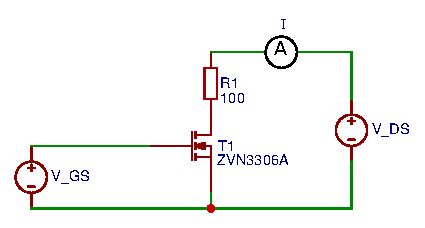
\includegraphics[width=\linewidth]{aufbau.pdf}
    \caption{Versuchsaufbau}
    \label{versuchsaufbau}
\end{figure}
Das erste Netzteil wurde am Transistor mit dem Gate-Source-Eingang verbunden und die Spannung zur Feststellung der Eingangskennlinie schrittweise erhöht. Am Drain-Source Eingang wurde ein weiteres Netzteil angeschlossen, an welchem die Spannung zur Festlegung der Ausgangskennlinie schrittweise erhöht wurde. Am jeweils anderen Netzteil wurde die Spannung konstant gelassen und ggf. nachgeregelt. Im Drain-Source Schaltkreis wurde ein Widerstand und das Ampermeter in Reihe geschaltet. Der Aufbau ist in \autoref{versuchsaufbau} zu sehen.
\subsection*{Verwendete Bauteile}
Multimeter, N-MOS Transistor ZVN3306A, $100 \Omega$ Widerstand, zwei Netzteile mit begrenztem Strom von $0.1 A$.
\section*{Durchführung}
Im ersten Versuchsteil sollte die Eingangskennlinie des Transistors (hier N-MOS) bestimmt werden. Dazu wurde die Drain-Source Spannung konstant bei $U_{DS} = 3 V$ gehalten und die Gate-Source Spannung schrittweise erhöht, während der Strom im Drain-Source Schaltkreis gemessen wurde. Beendet wurde die Messung, konnte keine signifikante Veränderung des Stroms festgestellt werden.
Im zweiten Teil wurde die Ausgangskennlinie erfasst, indem die Gate-Source Spannung konstant gehalten wurde, während die Drain-Source Spannung schrittweise erhöht wurde. Der Versuch wurde für zwei verschiedene, aber konstante, Gate-Source Spannungen durchgeführt, $U_{GS} = 3 V$ und $U_{GS} = 2.5 V$.
In beiden Teilen war mit jeder Spannungsveränderung darauf zu achten, dass die konstante Spannung gegebenenfalls nachjustiert werden musste.
\section*{Messergebnisse}
Für niedrige Spannungen im Gate-Source Kreis war kein Stromfluss zu erkennen, daher wurden die Messergebnisse zwischen $U_{GS} = 0.2 V$ und $U_{GS} = 1.9 V$
vernachlässigt. Hier ist ein Stromfluss von $I = 0 mA$ anzunehmen. Die Vollständigen Messergebnisse der Eingangskennlinie sind in \autoref{eingangskennlinie} zu finden. Die Daten sind graphisch in \autoref{graphEingangskennlinie} dargestellt.
\begin{table}[h]
\centering
\begin{tabular}{c|c}
$U_{GS} [V]$ & $I [mA]$ \\ \hline
$0$ 	& $0$ \\
$0.1$ 	& $0$ \\
$0.2$ 	& $0$ \\
$1.9$	& $0.241$ \\
$2.0$	& $0.67$ \\
$2.1$	& $1.518$ \\
$2.2$	& $3.054$ \\
$2.3$	& $5.162$ \\
$2.4$	& $7.765$ \\
$2.5$	& $10.96$ \\
$2.6$	& $14.28$ \\
$2.7$	& $17.83$ \\
$2.8$	& $21.37$ \\
$2.9$	& $23.34$ \\
$3.0$	& $24.1$ \\
$3.1$	& $24.5$ \\
$3.2$	& $24.72$
\end{tabular}
\caption{Messung der Eingangskennlinie}
\label{eingangskennlinie}
\end{table}
\begin{figure}[H]
    \centering
    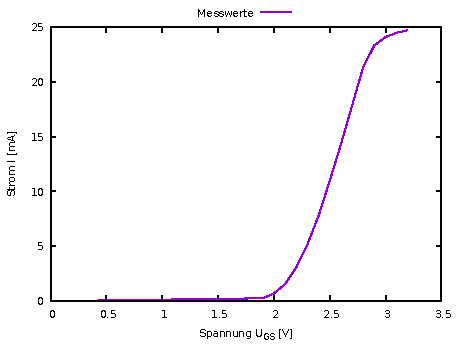
\includegraphics[width=\linewidth]{eingang.pdf}
    \caption{Eingangskennlinie mit $U_{DS}=3V$}
    \label{graphEingangskennlinie}
\end{figure}
\begin{figure}[H]
    \centering
    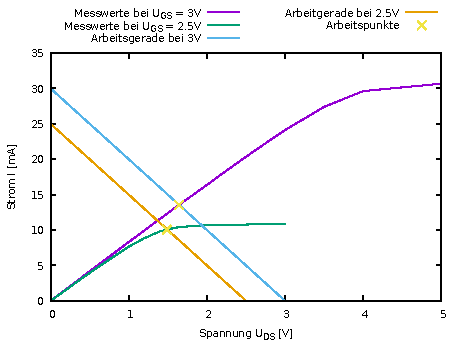
\includegraphics[width=\linewidth]{ausgang.pdf}
    \caption{Ausgangskennlinien}
    \label{graphAusgangskennlinie}
\end{figure}
Zur Bestimmung der Ausgangskennlinie wurde die Gate-Source Spannung auf $U_{GS} = 3 V$ im ersten, und auf $U_{GS} = 2.5 V$ im zweiten Durchgang geregelt. Die Messwerte sind in \autoref{ausgang3V} und \autoref{ausgang2-5V} zu finden und in \autoref{graphAusgangskennlinie} grafisch aufbereitet.
\begin{table}[htb]
    \centering
    \begin{minipage}[b][][b]{0.45\linewidth}
        \centering
		\begin{tabular}{c|c}
		$U_{DS} [V]$ & $I [mA]$ \\ \hline
		$0.0$ & $0.0$ \\
		$0.2$ & $1.59$ \\
		$0.4$ & $3.178$ \\
		$0.6$ & $4.729$ \\
		$0.8$ & $6.193$ \\
		$1.0$ & $7.644$ \\
		$1.2$ & $8.857$ \\
		$1.4$ & $9.821$ \\
		$1.6$ & $10.34$ \\
		$1.8$ & $10.56$ \\
		$2.0$ & $10.66$ \\
		$2.5$ & $10.79$ \\
		$3.0$ & $10.90$ 
		\end{tabular}
		\caption{Messung der Ausgangskennlinie bei $U_{GS} = 3 V$}
		\label{ausgang3V}
    \end{minipage}% 
    \hfill
    \begin{minipage}[b]{0.45\linewidth}
        \centering
		\begin{tabular}{c|c}
		$U_{DS} [V]$ & $I [mA]$ \\ \hline
		$0.0$ & $0.0$ \\
		$0.2$ & $1.666$ \\
		$0.4$ & $3.334$ \\
		$0.6$ & $5.0$ \\
		$0.8$ & $6.656$ \\
		$1.0$ & $8.314$ \\
		$1.2$ & $9.949$ \\
		$1.4$ & $11.58$ \\
		$1.6$ & $13.22$ \\
		$1.8$ & $14.78$ \\
		$2.0$ & $16.38$ \\
		$2.2$ & $18.0$ \\
		$2.4$ & $19.56$ \\
		$2.6$ & $21.13$ \\
		$2.8$ & $22.64$ \\
		$3.0$ & $24.13$ \\
		$3.5$ & $27.41$ \\
		$4.0$ & $29.63$ \\
		$5.0$ & $30.67$
		\end{tabular}
		\caption{Messung der Ausgangskennlinie bei $U_{GS} = 2.5 V$}
		\label{ausgang2-5V}
    \end{minipage}
\end{table}

\subsection*{Beobachtungen}
Auffällig war beim Bestimmen der Eingangskennlinie der rasche Anstieg des Stromes, sobald die Gate-Source Spannung eine gewisse Schwelle erreicht hatte.
Im Fall der Ausgangskennlinien ist zu bemerken, dass die Höhe, auf die sich der Strom bei höherem $U_{DS}$ einpendelt, scheinbar von der konstant gehaltenen Spannung $U_{GS}$ abhängt. Zudem lässt sich erkennen, dass der Ausgangsstrom exponentiell abhängig von $U_{DS}$ ist, bis hin zur einem gewissen Punkt, ab welchem der Strom sich auf einen gewissen Wert einpendelt

\section*{Auswertung}
Für $U_{GS} = 2.5 V$ lässt sich an der Grafik gut erkennen, dass zwischen $U_{DS} = 0 V$ und $U_{DS} = 1.4 V$ der Ausgangsstrom $I_D$ exponentiell ansteigt (in Abhängigkeit von $U_{DS}$). Dieser Bereich nennt sich Triodenbereich. Bei höheren $U_{DS}$ tritt dieser Effekt nicht mehr auf, der Strom pendelt sich bei $I_D = 11\si{\milli\ampere}$ ein im sogenannten Sättigungsbereich. \\
Die gleichen Beobachtungen lassen sich auch für $U_{GS} = 3 V$ machen, jedoch beginnt der Sättigungsbereich erst bei höherer Spannung von $U_{DS} = 4 V$ und erlaubt auch einen größeren Strom von $I_D = 32\si{\milli\ampere}$.

In \autoref{graphAusgangskennlinie} sehen wir zwei Ausgangskurven über der Drain-Source-Spannung, einmal bei festgehaltener Gate-Source-Spannung von $2.5V$ (a) und einmal $3V$ (b). In beiden Konfigurationen lässt sich der Graph in zwei Bereiche einteilen. Der Triodenbereich startet bei beiden Graphen bei $U_{DS} = 0 V$ und endet bei Konfiguration (a) bei ca. $U_{DS} = 1.5 V$. Bei Konfiguration (b) ist das Ende der Triodenbereich sehr viel höher mit rund $U_{DS} = 4.5 V$. In beiden Fällen startet ab diesem Punkt der Sättigungsbereich. Der größere Bereich im Falle einer Gate-Source Spannung von $3 V$ ist dadurch zu erklären, als dass, wie schon in dem ersten Versuchsteil gezeigt, die Leitfähigkeit ab $1.8 V$ bis $3.2 V$ exponentiell steigt. Damit kann bei einer Gate-Source Spannung von $2.5 V$ sehr viel weniger Strom fließen, als bei $3 V$.

\subsection*{Funktionsweise Transistoren$^{[1]}$}
\label{transistoren_info}

% subsection transistorunterschiede (end)}
\label{auswertung}
Der ZVN3306A ist ein N-Kanal-Transistor, der ZVP3306A ein P-Kanal Transistor. Daraus ergibt sich folgender wichtiger Unterschied: der N-Kanal-Transistor schaltet bei einer positiven Gate-Source-Spannung (sofern diese die Schwellspannung überwindet), der P-Kanal-Transistor hingegen schaltet nur bei einer negativen Gate-Source-Spannung. Dies ist bedingt durch den inneren Aufbau:
\\
\\
p-Kanal MOSFETs haben als Halbleiter zwischen Drain und Source ein n-dotiertes Metall, welches im Kristall-Gitter an manchen Stellen fünf-wertige Atome an Stelle der vier-wertigen Silicium-Atome besitzt. Dadurch gibt es an diesen Stellen einen Elektronenüberschuss; dieses zusätzliche Elektron ist frei beweglich. Wird jetzt am Bulk eine positive Spannung angelegt, so wird das Elektron zum Bulk hingezogen und und es entsteht ein Bereich mit positivem Potenzial am fünf-wertigen Atom. Dieses zieht andere, frei bewegliche Elektronen an und ermöglicht damit eine Ladungsträgerbewegung zwischen Drain und Source durch den Halbleiter.
\\
\\
Für n-Kanal MOSFETS sieht das ganze etwas anders aus. Das Halbleitermaterial ist p-dotiert, es wurden also fünf-wertige Atome in das vier-wertige Silicium gebracht. Der Effekt ist dadurch genau umgekehrt zu dem bei p-Kanal MOSEFETs: es gibt Elektronen-Lücken, die von freien Elektronen gefüllt werden können. Damit aber eine solche Lücke gefüllt wird, muss eine andere freigegeben werden. Dies lässt sich dann auch vereinfacht als bewegliche, positive Ladungsträger betrachten. Legen wir nun eine negative Spannung am Bulk an, so werden diese positiven Ladungsträger "aus dem Weg gezogen" und ein Stromfluss zwischen Drain und Source durch den Ladungsträger ist möglich.

\section*{Literaturverzeichnis}

[1] \nameref{transistoren_info}:
\url{https://lernraumplus.uni-bielefeld.de/pluginfile.php/117918/mod_resource/content/2/Skript%20Digitalelektronik%202018.pdf}     07.06.2018 10:20


\end{document}
